\begin{figure}[t]
\centering
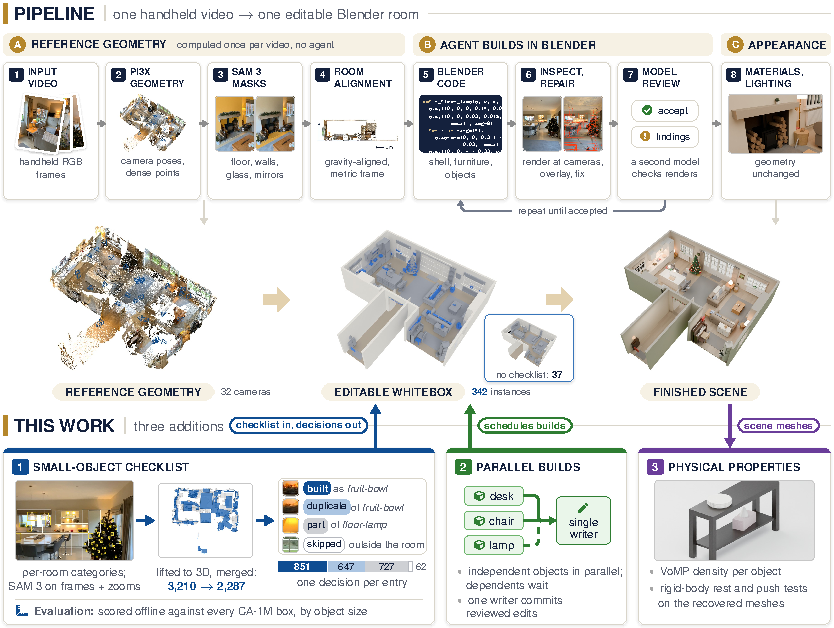
\includegraphics[width=\linewidth]{figures/system-pipeline.pdf}
\caption{\textbf{System overview.} Top: AHa-3D~\cite{aha3d} computes a
reference geometry from a handheld video, an agent authors the room in
Blender against renders from the video's cameras, and an optional pass adds
materials. Middle: one held-out room at each stage; instances under 50\,cm
are blue, and the inset is the same room built without the checklist.
Bottom: our additions, a detector checklist for small objects
(Section~\ref{sec:small-method}; the four entries are real, and the bar
counts the agent's decisions on all 2{,}287 entries of six held-out rooms),
concurrent object builds (Section~\ref{sec:architecture}) and physical
properties (Section~\ref{sec:physics-plan}).}
\label{fig:system}
\end{figure}
